\chapter{Theory}

To encompass all theory regarding stellar structure, evolution, and their
atmosphere is far beyond the scope of this thesis. Rather the theory needed is
presented below with highlights on the most important aspects.

\section{Stellar structure}

The structure of a non-rotating spherical stars can be described by five rather
simple differential equations \citep[see e.g.][]{kippenhahn} presented below:
\begin{enumerate}
    \item \textbf{Equation of Continuity}
        \nicebreak
        Relation between the mass, $m$, the density, $\rho$, at a symmetric
        shell at radius $r$
        \begin{align}
            \Aboxed{\pd{r}{m} &= \frac{1}{4\pi r^2\rho}.}
        \end{align}

    \item \textbf{Equation of Hydrostatic Equilibrium}
        \nicebreak
        The equation of hydrostatic equilibrium shows how a star in equilibrium
        is balanced between two forces. The inward force from gravity and the
        outward force from pressure, $P$,
        \begin{align}
            \Aboxed{\pd{P}{m} &= -\frac{Gm}{4\pi r^4}.}
        \end{align}
        When working with asteroseismology a time dependent perturbation to this
        equation is added \citep[see e.g.][for a thorough discussion]{Aerts2010}.
        However, this term is neglected here.


    \item \textbf{Equation of Energy Conservation}
        \nicebreak
        The equation of energy conservation shows how the energy is produced and
        lost throughout the star.
        \begin{align}
            \Aboxed{\pd{l}{m} = \epsilon - \epsilon_\nu + \epsilon_g,}
        \end{align}
        where $\epsilon$ is the energy production in the center of the star,
        $\epsilon_\nu$ is the energy lost by neutrinos which is always
        positive, $\epsilon_g$ is a source function of time-dependent terms,
        and $l$ is the luminosity at $m$. $\epsilon_g$ comes from the fact that
        non-stationary shells can change its internal energy, and thus exchange
        mechanical energy with neighboring shells.

    \item \textbf{Equation of Energy Transport}
        \nicebreak
        Energy transportation throughout the star is described with the
        following equation
        \begin{align}
            \Aboxed{\pd{T}{m} &= -\frac{GmT}{4\pi r^4P}\nabla_\tm{rad},}
        \end{align}
        where $\nabla_\tm{rad}$ is the radiative temperature gradient, and $T$
        is the temperature. The value of the temperature gradient compared to
        the radiative temperature gradient tells if the energy is transported by
        convection or radiation. In our Sun the outer layer are convective while
        the inner layer are radiative.

    \item \textbf{Equation of Chemical Composition}
        \nicebreak
        In this last equation we see the evolution of an element, $X_i$, when
        it reacts with other elements with reaction rates $r_{ji}$ and $r_{ik}$
        \begin{align}
            \Aboxed{\pd{X_i}{t} &= \frac{m_i}{\rho} \Bigl( \sum_j r_{ji} - \sum_k r_{ik}\Bigr).}
        \end{align}
        Note that this is the only time-dependent equation of the five
        presented.
\end{enumerate}

These five fundamental equations are implemented in stellar evolutionary codes,
which we will use in later chapters. The many different codes that exist take
other things into account, e.g the star can rotate, and it may not always be in
hydrostatic equilibrium (this is important if we want our star to pulsate). For
simplicity we have only presented time-dependence in the Equation of Chemical
Composition since timescales of rotation, pulsations, and activity are much
shorter than the long timescale found in chemical composition changes.


\section{Stellar atmosphere}

Much of this Section is inspired by \citet{Gray2006}. While all the figures here
were made by the author of this thesis, many of them can be found in
\citet{Gray2006} as well.

Write here about the formation of spectral lines...



\subsection{The equivalent width}

Measuring the equivalent width (EW) of spectral lines are important for some
analysis of stellar spectra. The EW is a measure of the strength of the line,
and dependent on the atmospheric conditions in where the spectral line is
formed, such as $T_\mathrm{eff}$, $\log g$, $[\ion{Fe}/\ion{H}]$, and
$\xi_\mathrm{micro}$.

\begin{figure}[htpb!]
    \centering
    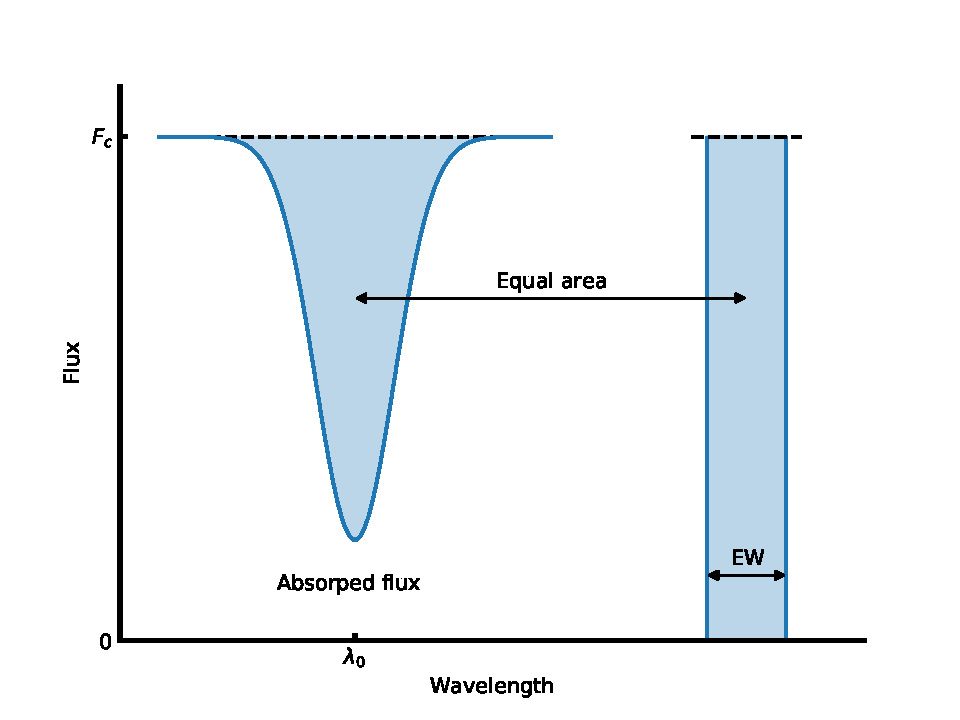
\includegraphics[width=1.0\linewidth]{figures/ewTheoretical.pdf}
    \caption{An absorption line centered at $\lambda_0$ normalized at the flux
             level $F_c$. The area of the absorption line to the left is equal
             to the blue shaded area in the rectangle to the right with width
             EW.}
    \label{fig:ewTheoretical}
\end{figure}

The EW is mathematically described as integrating over the entire line, and
assign this area to a rectangle from 0 to the continuum flux ($F_c$) with the
width, EW. This is illustrated in \fref{fig:ewTheoretical} and the equation
below: \begin{align} EW = \int_{0}^{\infty} \frac{F_c-F(\lambda)}{F_c} d\lambda,
\end{align} where $\lambda$ is the wavelength. This is integral is assuming
there is only one single line, hence the integral is over all wavelength. In
practice the integral is calculated in small windows around a spectral line. See
\sref{sec:measureEW} for more details on how this is performed in practice. The
unit of the EW is the same as the wavelength used. Throughout this thesis we
will use \AA{}ngstr\"{o}m (1\AA$=\SI{0.1}{nm}$) for the wavelength, and m\AA{}
for the EW.


\subsubsection{Temperature dependence}

As mentioned above the EW depends on the atmospheric parameters. The dependence
on $T_\mathrm{eff}$ is the strongest dependence. At low $T_\mathrm{eff}$ neutral
elements, say \ion{Fe}{I}, are the strongest lines as the number of ionized
atoms are too small to contribute significantly to the EW. As $T_\mathrm{eff}$
increases \ion{Fe}{I} is converted into ionized \ion{Fe}{II}. Slowly, as the
number of \ion{Fe}{I} decreases so does the EW, and likewise as the number of
\ion{Fe}{II} increases so does the EW. This goes on until second ionized atoms,
\ion{Fe}{III}, are formed and the same situation arise again. This is
illustrated in \fref{fig:ewTeff} where the EW of two iron lines, one neutral and
one ionized, are plotted against $T_\mathrm{eff}$. These two lines have similar
EW in the Sun: $\SI{46.2}{m}$\AA{} and $\SI{53.9}{m}$\AA{} for the \ion{Fe}{I}
and \ion{Fe}{II} line respectively.

\begin{figure}[htpb!]
    \centering
    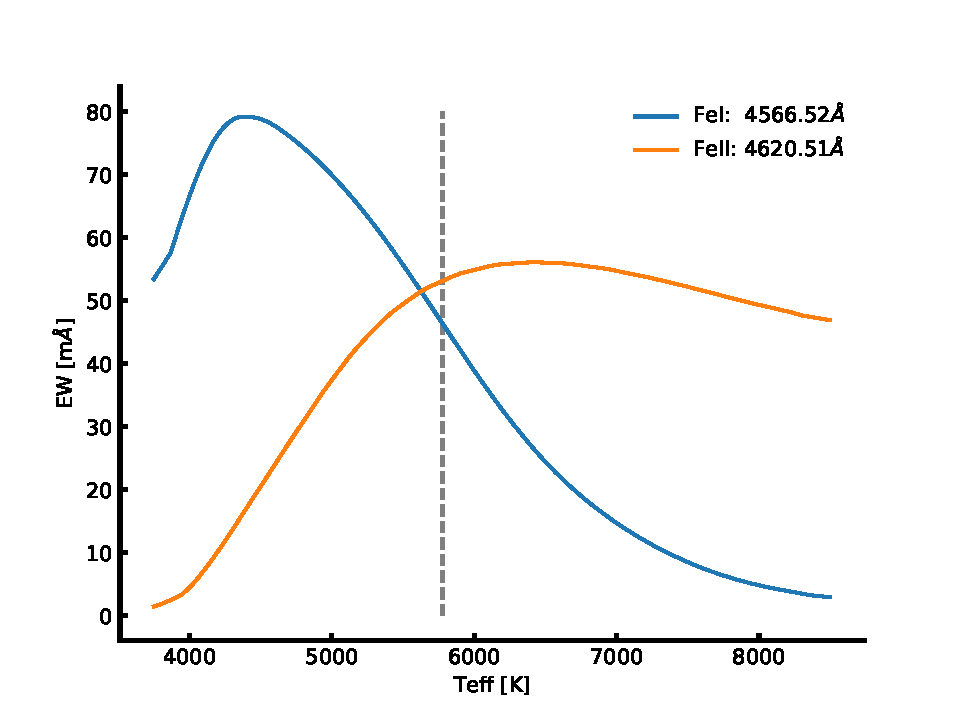
\includegraphics[width=1.0\linewidth]{figures/ewTeff.pdf}
    \caption{The EW for a \ion{Fe}{I} and \ion{Fe}{II} line with increasing
             $T_\mathrm{eff}$. The two lines have similar EW in the Sun and are
             found in the optical part of the spectrum.}
    \label{fig:ewTeff}
\end{figure}


\subsubsection{Pressure dependence}

Pressure dependence in the stellar atmosphere can be related to the gravity
dependence. There are many ways to measure the pressure, and thus the gravity
which is what is ultimately the goal with the measurement of $\log g$. Below are
listed some of the most common methods to measure $\log g$ from spectroscopy.

\begin{itemize}
  \item Continuum: The Balmer jump is the only continuum feature sensitive
        enough to estimate the $\log g$.
  \item Hydrogen lines: Hydrogen profiles are pressure sensitive and can
        therefore be used to estimate $\log g$. However, the gravity dependence
        rapidly diminishes for temperatures above $\SI{10\,000}{K}$.
  \item Other strong lines: There exists other strong lines with
        pressure-broadened wings such as the \ion{Ca}{II} H and K lines. These
        are better for cooler stars than the hydrogen lines described above.
  \item Weak lines: By comparing two stages of ionization for the same element
        it is possible to obtain $\log g$ using weaker or modestly strong lines.
\end{itemize}
In this thesis weak lines are used to measure $\log g$. More specifically a
comparison between \ion{Fe}{I} and \ion{Fe}{II} lines are used. For FGK stars,
as the atmosphere contracts (i.e. $\log g$ increases) the pressure likewise
increases, which in turn means that both the gas pressure, $P_g$, and electron
pressure, $P_e$, increases. Since hydrogen is the main electron contributor, but
not fully ionized for these stars, the electron pressure is much smaller that
the gas pressure. The gas pressure follow a simply emperical approximation with
gravity:
\begin{align}
  P_g \simeq \mathrm{constant}\, g^{2/3},
\end{align}
where $g$ is the gravity.



\begin{figure}[htpb!]
    \centering
    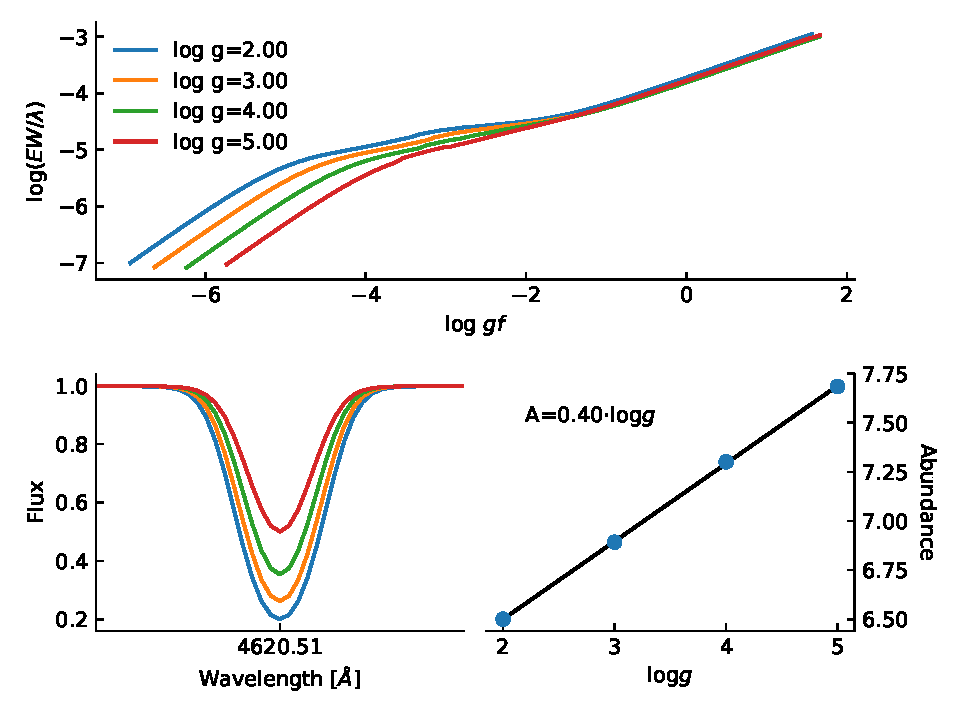
\includegraphics[width=1.0\linewidth]{figures/ewGravity.pdf}
    \caption{\emph{Upper panel}: Curve of growth for same \ion{Fe}{II} used in
             \fref{fig:ewTeff} for four different $\log g$ values. Here it is
             the weak lines mostly affected by the change in $\log g$.
             \emph{Lower left panel}: Synthetic spectra of the same line. The
             colour scale is the same.
             \emph{Lower right}: The abundance for the line at different
             $\log g$. A strong correlation (0.40) is seen.}
    \label{fig:ewGravity}
\end{figure}




\subsubsection{Abundance dependence}

The abundance of a given element obviously has an effect on the EW. The more
abundant an element is, the more photons can be absorbed thus increasing the EW.
However, the relationship is not strictly linear. For weak lines (GIVE RANGE) EW
is approximately linear with the abundance, however it reach a plateau where the
core of the line saturates. In this regime the EW only increases slowly, until
the absorption "spills" into the wings and the increase is again linear.
However, for these strong lines the shape is no longer Gaussian. The curve of
growth for the same \ion{Fe}{I} line used in \fref{fig:ewTeff} is shown in
\fref{fig:cog}. Instead of EW it is common to use the reduced EW, $\log
(EW/\lambda)$\footnote{The reduced EW is useful since it normalizes
Doppler-dependent phenomena, such as microturbulence and thermal broadening.},
which we will use more later. Instead of the abundance of a line, the oscillator
strength, $\log \mathit{gf}$, is used.

\begin{figure}[htpb!]
    \centering
    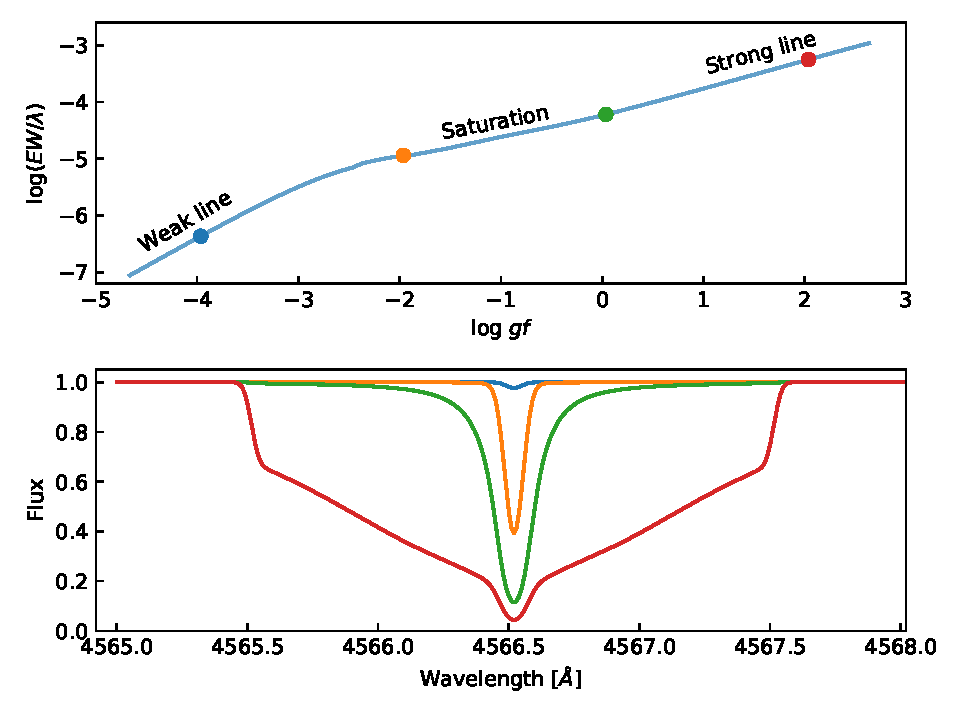
\includegraphics[width=1.0\linewidth]{figures/cog.pdf}
    \caption{\emph{Upper panel:} Curve of growth of the same \ion{Fe}{I} line as
             used in \fref{fig:ewTeff}. Four points are marked which is shown in
             the \emph{lower panel} as a synthetic spectral line. The RW (proxy
             for EW) is clearly increasing with $\log \mathit{gf}$ (proxy for
             abundance).}
    \label{fig:cog}
\end{figure}


\subsubsection{Microturbulence}

Small-scale motion, that is motion of material at length scales small compared
to the unit optical depth, are called microturbulence, $\xi_\mathrm{micro}$.
This is not to be confused with macroturbulence, which is motion of material at
scales larger than the unit optical depth. The latter is associated with
granulation and will not be discussed further in this thesis.
$\xi_\mathrm{micro}$ comes into play when looking at the curve of growth for
saturated lines (i.e. between green and red points in \fref{fig:cog}). If no
$\xi_\mathrm{micro}$ is assumed, then the measured abundance is higher than
predicted by models based on thermal and damping broadening alone. In
\fref{fig:cog_vt} is shown three curves of growth with
$\xi_\mathrm{micro}={\SI{0.5}{km/s}, \SI{2.5}{km/s}, \SI{5.0}{km/s}}$. As
$\xi_\mathrm{micro}$ increases, so does the EW and hence the abundance.

\begin{figure}[htpb!]
    \centering
    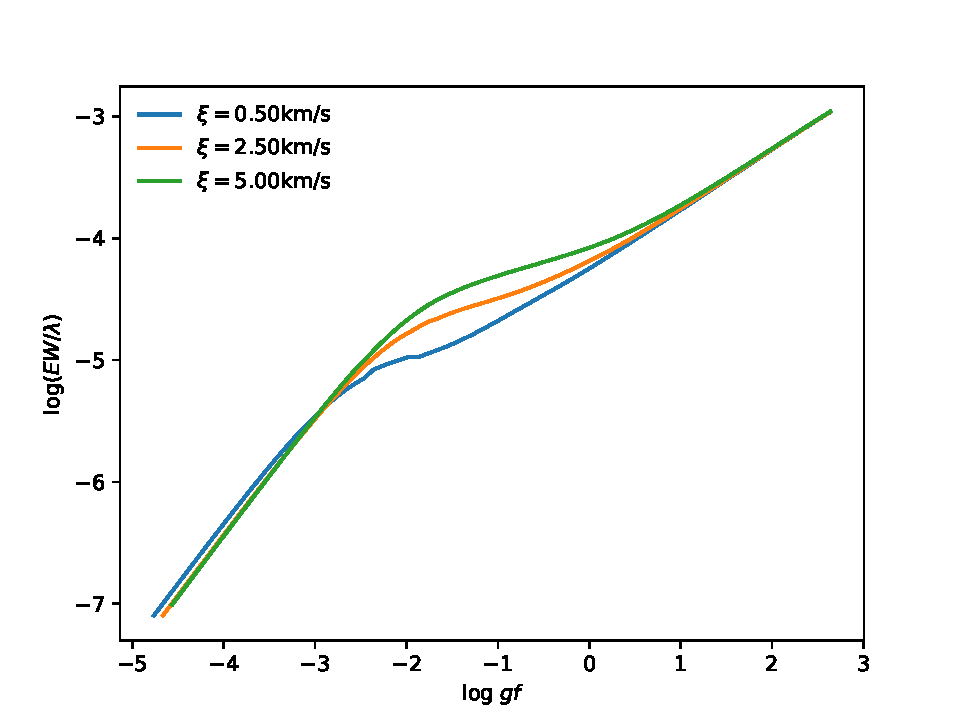
\includegraphics[width=1.0\linewidth]{figures/cog_vt.pdf}
    \caption{Curve of growth for three different values of $\xi_\mathrm{micro}$.
             The EW is increasing with increasing $\xi_\mathrm{micro}$.}
    \label{fig:cog_vt}
\end{figure}

The broadening of an absorption line measured by the shift in wavelength,
$\Delta\lambda$, when $\xi_\mathrm{micro}$ is included is defined as:
\begin{align}
  \Delta\lambda = \frac{\lambda_0}{c} \sqrt{\frac{2kT}{m} + \xi_\mathrm{micro}^2},
\end{align}
where $c$ is the speed of light, $\lambda_0$ is the rest wavelength of the given
line, $k$ is Boltzmann's constant, $T$ is the temperature, and $m$ is the mass
of the atom. Setting $\xi_\mathrm{micro}=\SI{0}{km/s}$, we end up with thermal
broadening.


\subsection{Stellar parameters for FGK stars}

\subsubsection{Line list and atomic data}

\subsubsection{Measuring EW}
\label{sec:measureEW}

\subsubsection{Determining abundances with MOOG}
